% Kapitel 3 mit den entsprechenden Unterkapiteln
% Die Unterkapitel können auch in separaten Dateien stehen,
% die dann mit dem \include-Befehl eingebunden werden.
%-------------------------------------------------------------------------------
\chapter{Implementierungsentwurf}

In diesem Kapitel werden die Implementierungsdetails für die Umsetzung des
Grobentwurfs vorgestellt. Gegenüber letzterem werden neben den Schnittstellen
auch die Implementierungen spezifiziert. Die Abbildungen zeigen die 
Klassenhierachie in den jeweiligen Paketen. Aus Gründen der Übersichtlichkeit
wird in den Implementierungen auf die Auflistung der Operationen der Schnittstellen
verzichtet.

\begin{figure}[!h]
	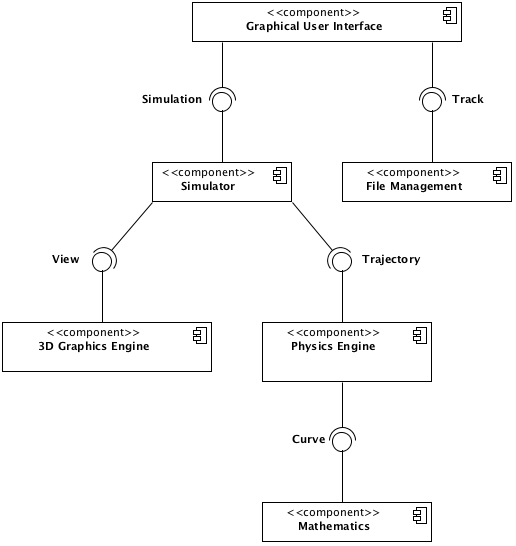
\includegraphics[width=0.8\linewidth]{bilder/components.png}
\caption{Komponentendiagramm}
\end{figure}


\section{Gesamtsystem}
Fügen Sie hier bitte das Komponentendiagramm aus dem Grobentwurf ein und
erläutern Sie kurz die Funktionen der Komponenten.
%%%%%%%%%%%%%%%%%%%%%%%%%%%%%%%%%%%%%%%%%%%%%%%%%%%%%%%%%%%%
\section{Implementierung von Komponente
         <ID aus Grobentwurf>: <Komponentenname>:}

Beschreiben Sie hier bitte die Implementierung der Komponente. Erläutern Sie
bitte dabei, welche Entwurfsmuster und Bibliotheken Sie verwenden. Die
Implementierung wird dabei durch Klassendiagramme dokumentiert.

\subsection{Paketdiagramm}
\subsection{Erläuterung}

Die verwendeten Attribute, Aufgaben und Kommunikationspartner sind für jede
Klasse kurz zu erläutern. Die ankommenden Nachrichten beziehen sich dabei auf
die Sequenzdiagramme der Feinanalyse im Grobentwurf und stellen meist
aufzurufende Methoden der Klasse dar.  Reine get- / set-Methoden oder
Bibliotheksfunktionen brauchen nicht aufgeführt zu werden.


%%%%%%%%%%%%%%%%%%%%%%%%%%%%%%%%%%%%%%%%%%%%%%%%%%%%%%%%%%%%
\section{Implementierung von Komponente
         Graphics3D: 3D-Anzeige:}

Die  3D-Anzeige-Komponente übernimmt die dreidimensionale Visualisierung der Achterbahn
mit Gerüst und Umgebung.Sie kapselt die allgemeinen gehaltenen Funktionen der eingesetzten
Grafikbibliothek JMonkeyEngine und stellt eine einfache Schnittstelle für das Befüllen 
der virtuellen Welt mit Achterbahnkomponenten sowie zur Steuerung der Kamerafahrten 
entlang der befahrenen Strecke zur Verfügung.

\textbf {Dieser Bereich ist noch nicht entgültig fertig,bedarf einer Überarbeitung und steht zur Diskussion!}

\begin{figure}
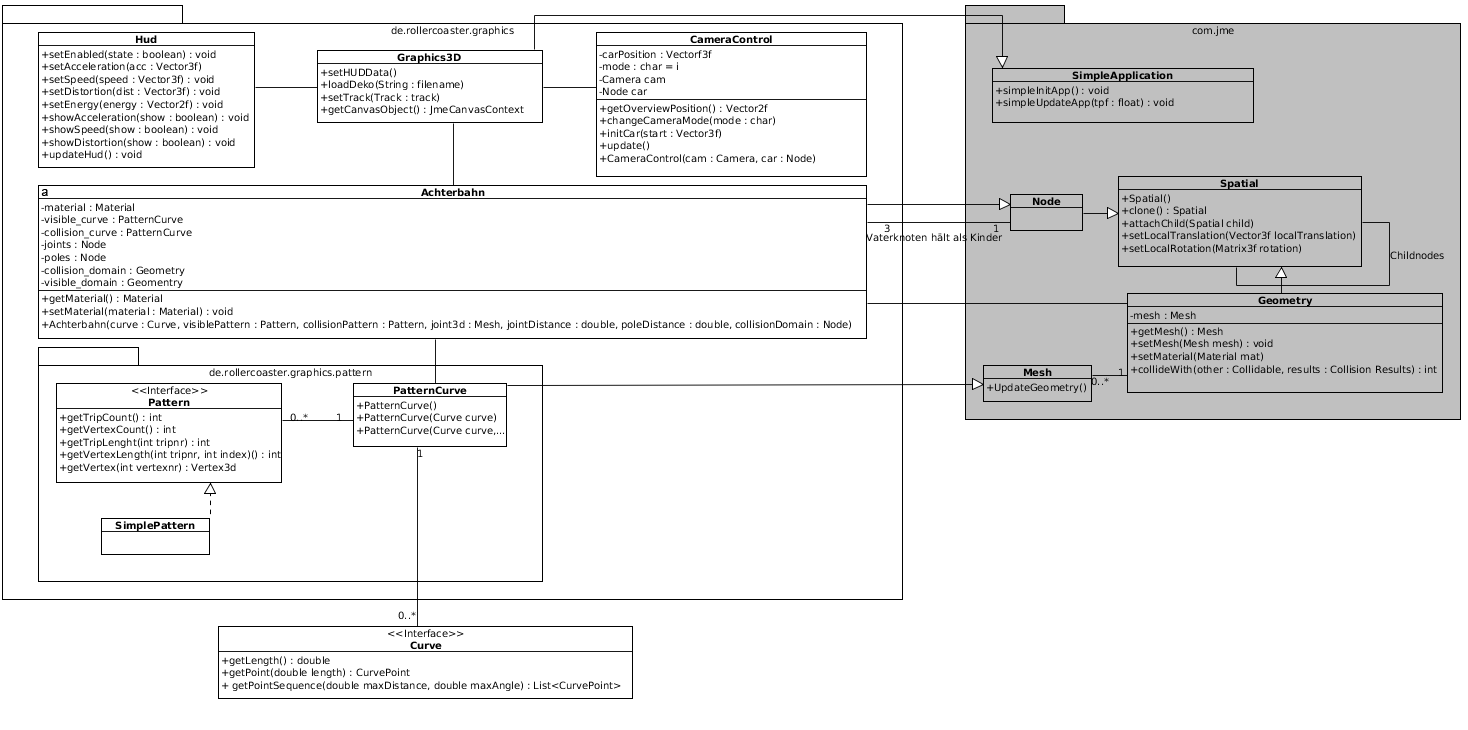
\includegraphics[width=\linewidth]{bilder/klassendiagramm_006}
\caption{Klassendiagramm Graphics3D}
\end{figure}

Graphics3D erbt von SimpleApplication und stellt einen 3D-Kontext zur Verfügung der in die 2DGui eingebunden wird. Außerdem sorgen die simpleInit Methode für die Einrichtung aller Geometrien soweit es zur Startzeit möglich ist.
Die JMonkeyEngine stellt eine Scenegraphenstruktur über Spatial zur Verfügung die hier kurz skizziert wird. Die Subklassen Geometry als Meshcontainer und Node als Strukturelement werden von unserer Klasse Achterbahn 
zur Speicherung und Ordnung der Geometrieelemente verwendet. Mittels setTrack wird eine dabei ein Track übergeben der die Bahndaten einer Achterbahn enthält, die dann umgerechnet werden kann. PatternCurve ist eine Klasse die ein Pattern entlang einer Curve extrudiert. 
Damit werden die Schienen anhand eines Profils (Pattern) entlang der Kurve erzeugt. 

Auf die von der JMonkeyengine bereitgestellte Zeichenfl"ache wird ein \textsl{Head up Display} projeziert. Dieses dient dazu dem Benutzer einen schnellen 
"Uberblick "uber den  aktuellen Status der Simulation zu erlauben, ohne erst die Messwerte numerisch auswerten zu m"ussen. Dem \textsl{HuD} können verschiedene Werte zur
Anzeige "ubergeben werden.

Um zusätzliche unterschiedliche Sichtmodi zur Verfügung zu stellen existiert die Kameraklasse. In CameraControl wird über den Konstruktor ein Camera Objekt und ein Knoten übergeben. Das Camera Objekt wird bei changeCameraMode verändert, wie in der 2D-GUI festgelegt, also Wechsel zwischen overview und interior view. Diese Änderung wird sofort in der update Methode berücksichtigt, sodass die Kamera-Änderung aktualisiert wird ohne die Achterbahnfahrt zu stoppen. Die getOverwiePosition Methode gibt einen 2D-Vektor zurück, um auf der Übersichtskarte im HUD die Position in 2D anzuzeigen. Dort wird also der 3d Vektor carPosition in einen 2D Vektor umgerechnet.


\begin{figure}
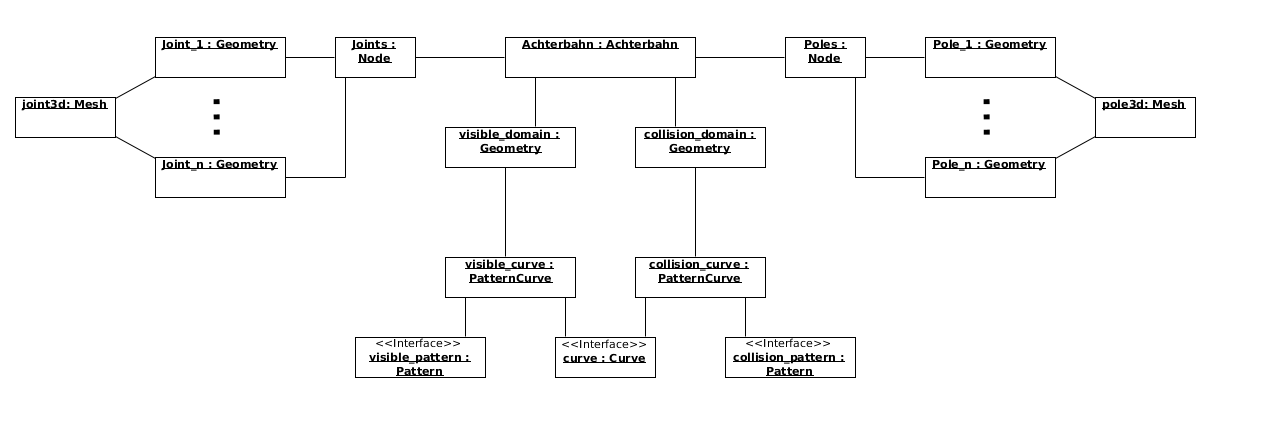
\includegraphics[width=\linewidth]{bilder/objektdiagramm_004}
\caption{Objektdiagramm Achterbahn}
\end{figure}

Im wesentlichen hält die Achterbahn 4 Knoten. Unter joints hängen alle n Geomentrien die auf die gleiche Mesh zeigen und die Verbindungsstücke der Bahn erzeugen. Das Konzept erlaubt, dass in jedem Geometry eigene Rotation und 
Translation gesetzt werden, sodass die Mesh an unterschiedlichen Orten im 3D-Raum gezeichnet wird, ohne jedoch die Mesh im Speicher vollständig kopieren zu müssen. Poles enthält die Stützpfeiler der Bahn und ist analog strukturiert.
Die Schienen werden in der visible\_domain durch eine PatternCurve erzeugt. In der collision\_domain liegt eine zweite PatternCurve, die ein BoundingVolume um die Bahn definiert um Kollisionen mit bereits geladener oder neu zu ladener
Dekoration zu erkennen. Dieses BoundingVolume wird außerdem dazu verwendet die Stützpfeiler zu generieren, ohne dass diese in durch die Bahn ragen.

% \begin{figure}
%   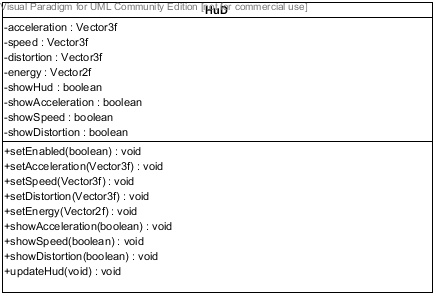
\includegraphics[width=0.8\linewidth]{bilder/HuD.png}
%  \caption{Head up Display}
% \end{figure}


\subsection{Paketdiagramm}
\subsection{Erläuterung}

Die verwendeten Attribute, Aufgaben und Kommunikationspartner sind für jede
Klasse kurz zu erläutern. Die ankommenden Nachrichten beziehen sich dabei auf
die Sequenzdiagramme der Feinanalyse im Grobentwurf und stellen meist
aufzurufende Methoden der Klasse dar.  Reine get- / set-Methoden oder
Bibliotheksfunktionen brauchen nicht aufgeführt zu werden.

%%%%%%%%%%%%%%%%%%%%%%%%%%%%%%%%%%%%%%%%%%%%%%%%%%%%%%%%%%%%
\section{Implementierung von Komponente
         <ID aus Grobentwurf>: Benutzeroberfläche:}

Die grafische Benutzeroberfläche übernimmt die Interaktion zwischen dem Benutzer und
der Simulation. Dazu gehört die Steuerung des Hauptmenüs, des Dateidialoges und
des Optionen-Dialogs. Die aus der Dateiverwaltung ausgelesenen Achterbahn-Kurven 
werden an den Simulator zur Darstellung übergeben. Die Nutzeraktionen bezüglich des
Simulationsablaufes werden durchgereicht. Die Benutzeroberfläche lässt sich über
Änderungen am physikalische Zustand des Achterbahnwaagens informieren und stellt
wichtige Daten grafisch dar.

\subsection{Paketdiagramm}
\subsection{Erläuterung}

Die verwendeten Attribute, Aufgaben und Kommunikationspartner sind für jede
Klasse kurz zu erläutern. Die ankommenden Nachrichten beziehen sich dabei auf
die Sequenzdiagramme der Feinanalyse im Grobentwurf und stellen meist
aufzurufende Methoden der Klasse dar.  Reine get- / set-Methoden oder
Bibliotheksfunktionen brauchen nicht aufgeführt zu werden.

%%%%%%%%%%%%%%%%%%%%%%%%%%%%%%%%%%%%%%%%%%%%%%%%%%%%%%%%%%%%
\section{Implementierung von Komponente
         <ID aus Grobentwurf>: Dateiverwaltung:}

Die Dateiverwaltungs-Komponente übernimmt das Einlesen der Achterbahn-Spezifikationen 
aus den vom Editor bereitgestellten XML-Dateien. Alle speziellen Eigenheiten des
eingesetzten Serialisierung-Schema werden gekapselt. Den übrigen Komponenten wird 
lediglich eine glatte Raumkurve und ein Satz einfach auslesbarer Parameter zur Verfügung
gestellt.

\subsection{Paketdiagramm}

\begin{figure}
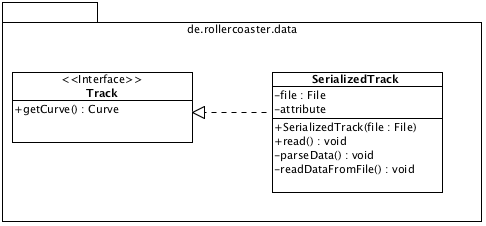
\includegraphics[width=\linewidth]{bilder/Data}
\caption{Daten}
\end{figure}

\subsection{Erläuterung}

Die Schnittstelle \emph{Track} wird durch die Klasse \emph{SerializedTrack} realisiert,
welche im Konstruktor die Spezifikationsdatei als Argument übergeben bekommt. Über
die Methode \emph{read} wird das Auslesen der Spezifikation veranlasst, wobei
die Hilfsfunktionen \emph{readDataFormFile} und \emph{parseData} zum Einsatz kommen.

%%%%%%%%%%%%%%%%%%%%%%%%%%%%%%%%%%%%%%%%%%%%%%%%%%%%%%%%%%%%
\section{Implementierung von Komponente
         <ID aus Grobentwurf>: Mathematik}

Die Mathematik-Komponente stellt Routinen zur näherungsweisen Berechnung
von Beziérkurven, dem Lösen von gewöhnlichen Differentialgleichungen 
(Anfangswertproblemen) und Algorithmen zum Lösen von linearen Gleichungssystemen
zur Verfügung. Dadurch ist es möglich, aus einer über Stützstellen definierte 
Achterbahn in eine glatte Raumkurve umzurechnen und die Bewegung auf
der Bahnkurve durch numerische Integration zu bestimmen.

\subsection{Paketdiagramm}

\begin{figure}
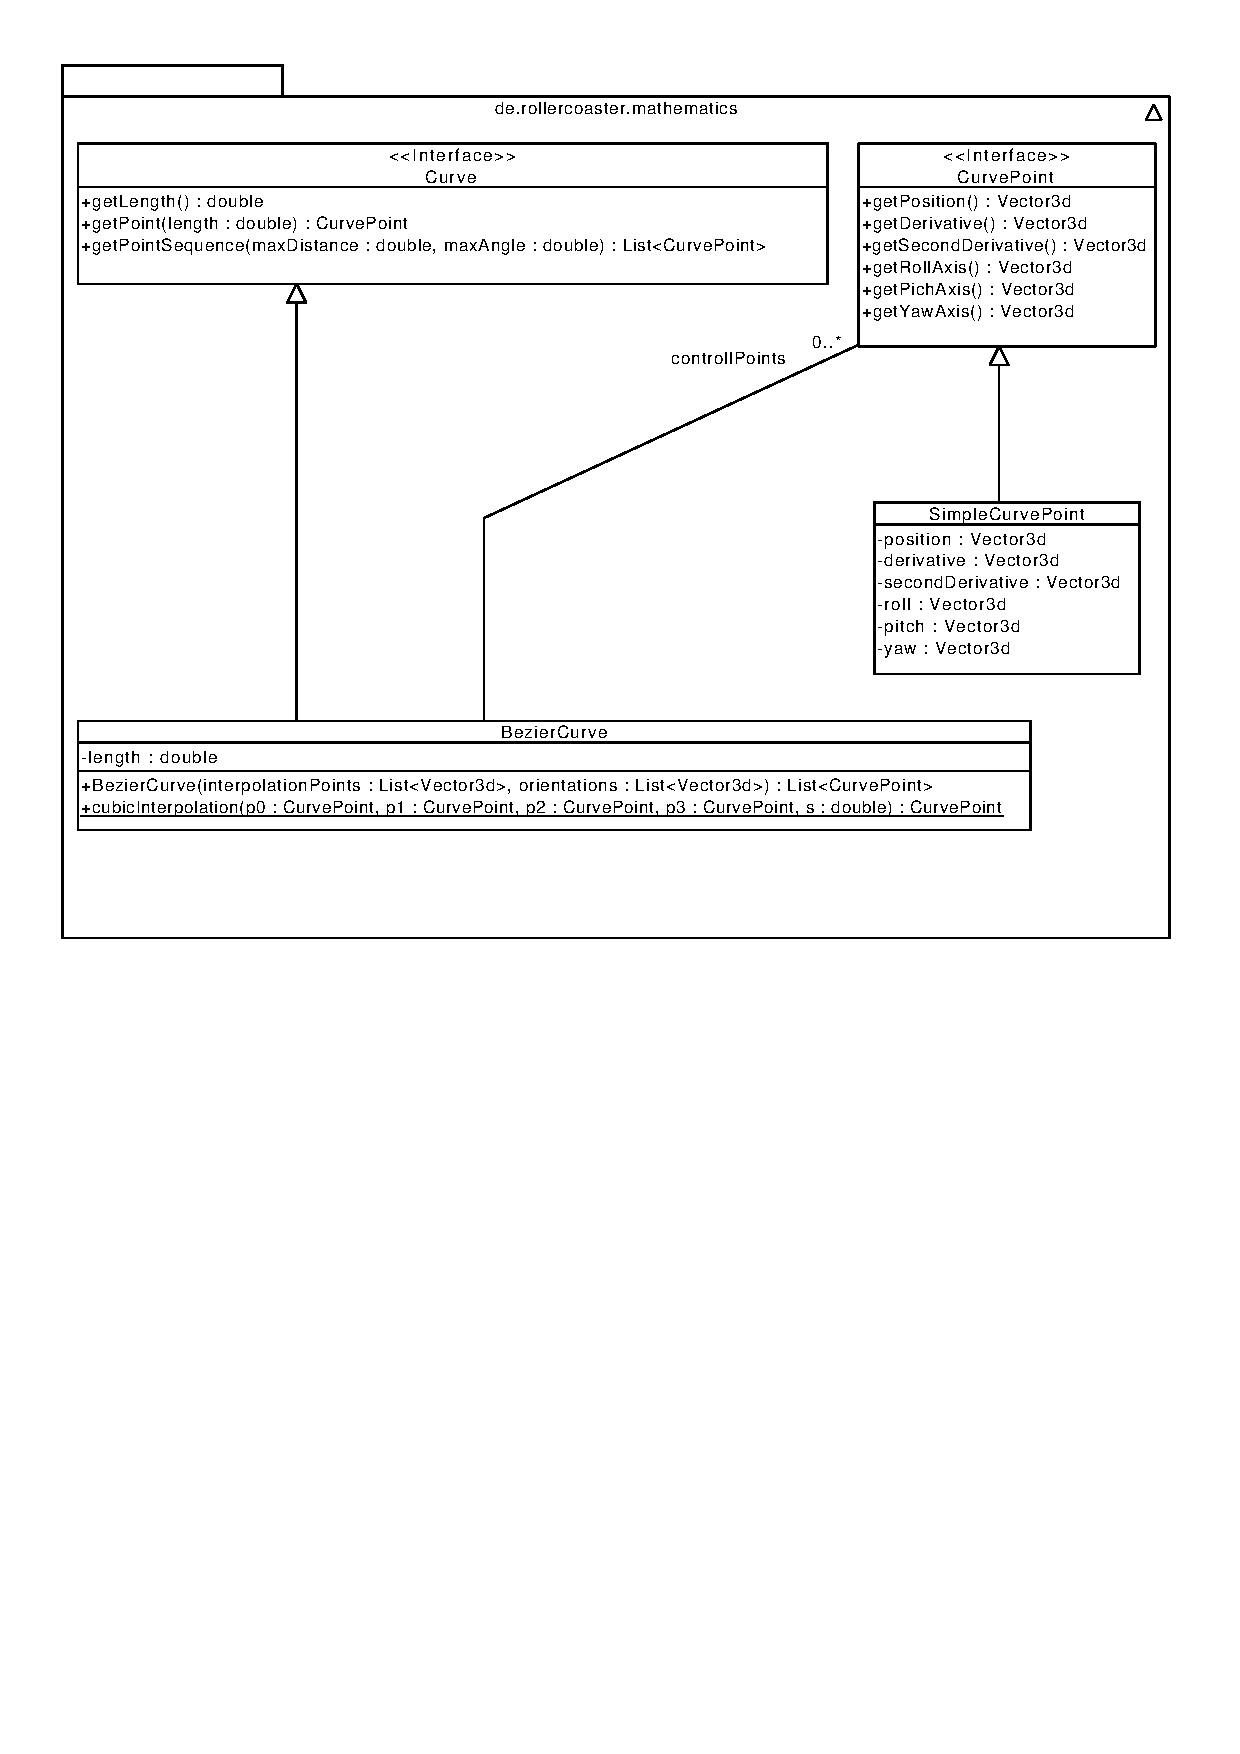
\includegraphics[width=\linewidth]{bilder/Mathematics}
\caption{Mathematik (Raumkurven)}
\end{figure}
\begin{figure}
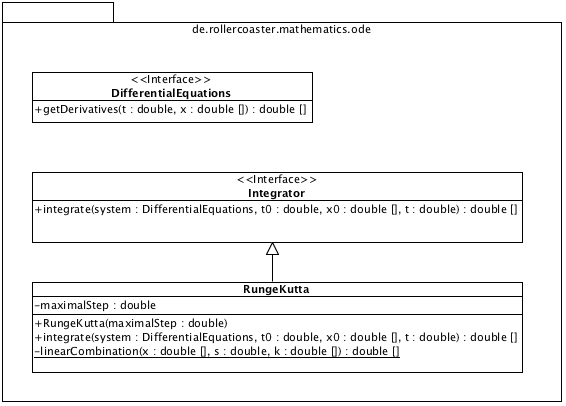
\includegraphics[width=\linewidth]{bilder/Mathematics_ODE}
\caption{Mathematik (Diffentialgleichungen)}
\end{figure}

\subsection{Erläuterung}
Die Schnittstelle \emph{Curve} für Raumkurven wird durch die Klasse \emph{BezierCurve} 
realisiert,welche im Konstruktor eine Liste mit Stützstellen und eine Liste mit der
räumlichen Orientierung auf den Stützstellen als Argumente übergeben bekommt. Die Bahn
ist bei dieser Implementierung glatt: wenn immer eine Zwischenstelle angefordert wird,
erfolgt eine kubische Interpolation über die statische Methode \emph{cubicInterpolation}.
Diese Methode bekommt die vier benachbarten Kontrollpunkte und einen Bahnparameter $s$
übergeben und interpoliert die Position, die Orientierung sowie die ersten beiden 
Ableitungen der Raumkurve. 
Die Punkte auf der Raumkurve werden durch die Schnittstellenklasse \emph{CurvePoint}
repräsentiert, welche mit \emph{SimpleCurvePoint} eine Realisierung als einfache
Speicherklasse ohne weitere Funktionalität bekommen hat.

Für die Lösung der Differentialgleichungen wurden gegenüber des Grobentwurfs ein
weitere Teilkomponente spezifiziert. Das Gleichungssystem wird über die Schnittstelle
\emph{DifferentialEquations} repräsentiert, das Lösungsverfahren über die Schnittstelle
\emph{Integrator}. Der Integrator bekommt ein Gleichungssystem, den aktuellen Zustand
der unabhängigen und abhängigen Variablen (Zeit und Bahnparameter) und das gewünschte
Ziel übergeben. Je nach Lösungsverfahren werden ein- oder mehrere Auffrufe für die
Berechnung der rechten Seite des Diffentialgleichungssystem über die Methode 
\emph{getDerivatives} durchgeführt, aus denen der Endzustand interpoliert wird.
Als Realisierung wird \emph{RungeKutta} umgesetzt, welche eine lineare Interpolation
\emph{linearCombination} als Hilfsmethode benötigt.

%%%%%%%%%%%%%%%%%%%%%%%%%%%%%%%%%%%%%%%%%%%%%%%%%%%%%%%%%%%%
\section{Implementierung von Komponente
         <ID aus Grobentwurf>: Physik:}

In der Physik-Komponente erfolgt die Berechnung der Achterbahnbewegung. Dazu wird
die Bewegung eines Massenpunktes auf der von Außen vorgegebenen Raumkurve
nach den Gesetzen der klassischen Mechanik bestimmt. Die Berechnung erfolgt
durch numerisches Lösen einer gewöhnliche Differentialgleichung, welche von der
Physik-Komponente repräsentiert und von der Mathematik-Komponente integriert wird.
Für jeden Zeitschritt wird der Zustand des Massenpunktes aktualisiert und an die
übergeordneten Komponenten weitergereicht.

\subsection{Paketdiagramm}
\begin{figure}
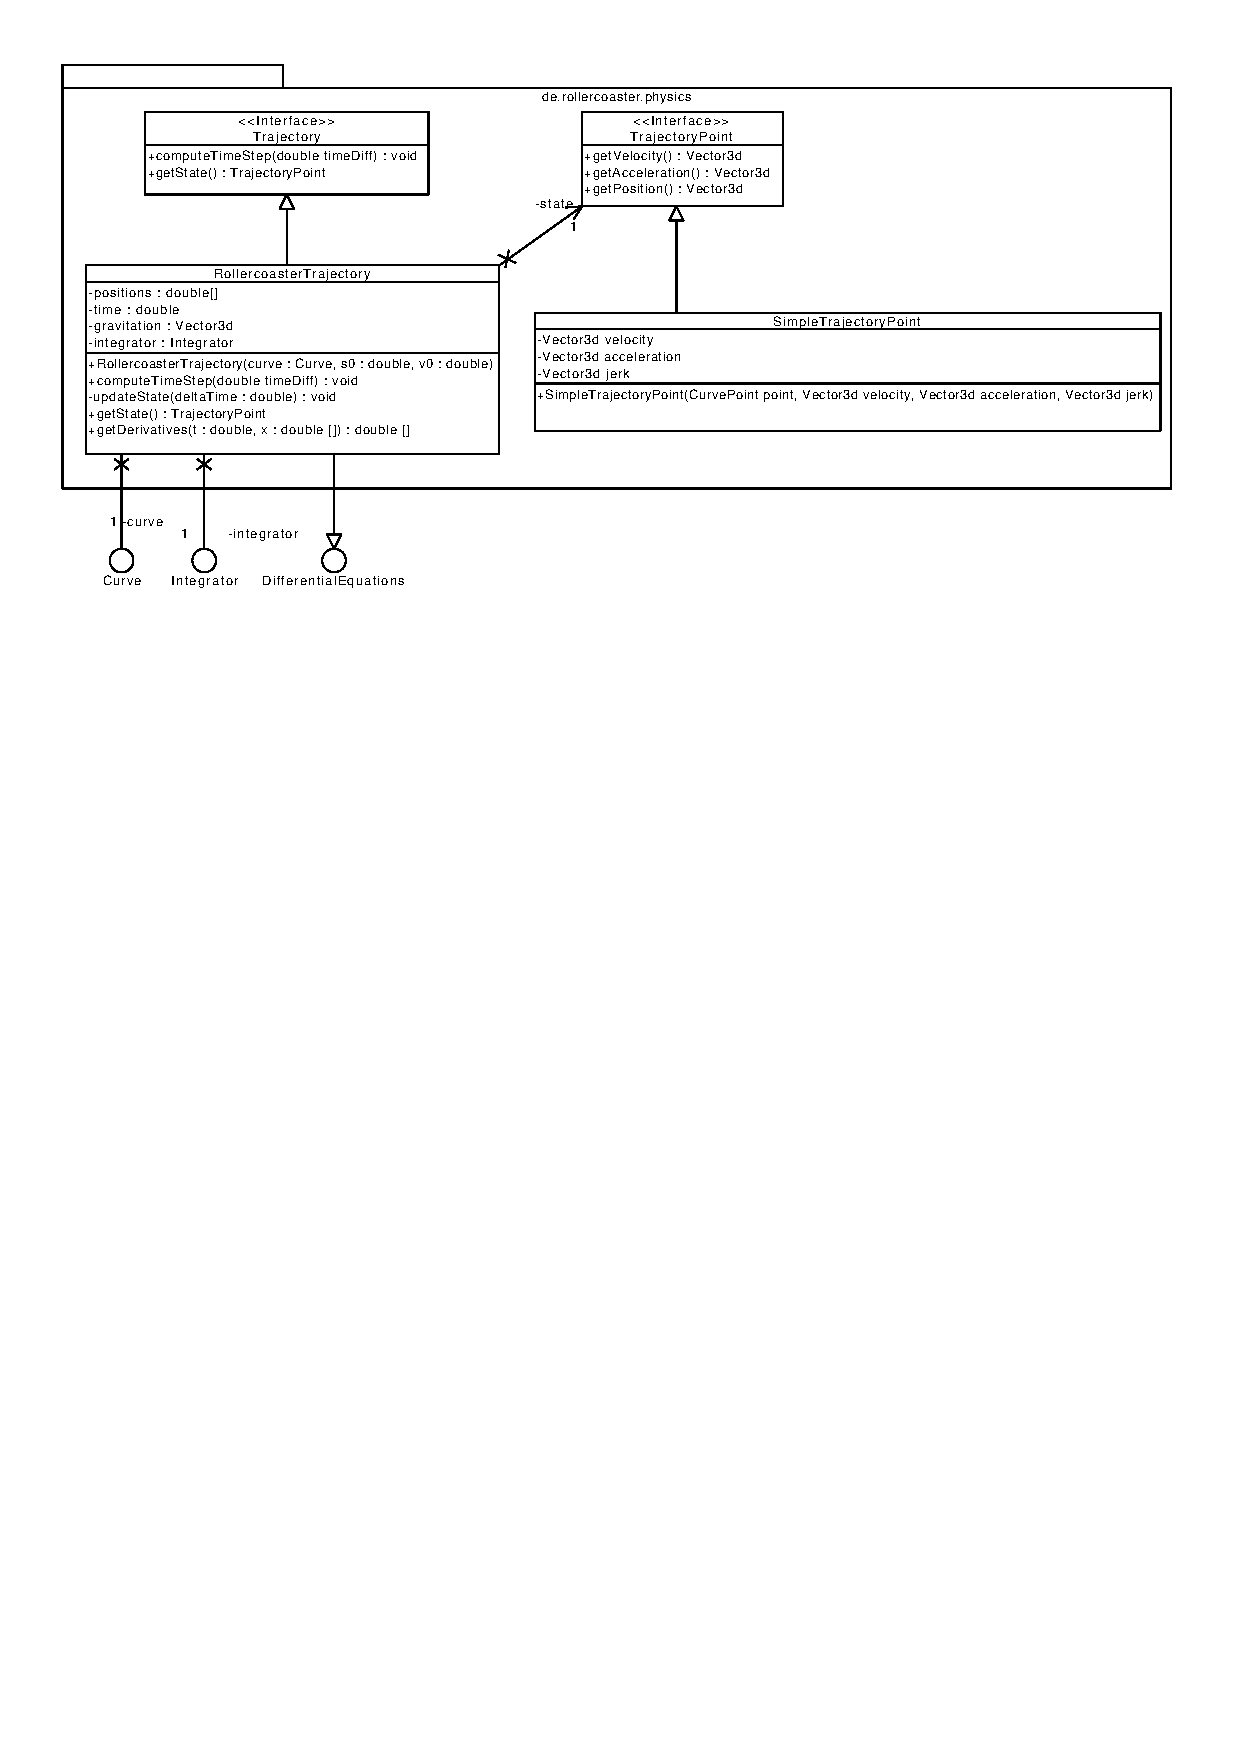
\includegraphics[width=\linewidth]{bilder/Physics}
\caption{Physik}
\end{figure}

\subsection{Erläuterung}

Die Entwicklung des physikalischen Systems wird als Bahnkurve durch die Schnittstelle
\emph{Trajectory} zusammengefasst. Dabei wird für diskrete Zeitpunkte jeweils ein
Zustand als \emph{TrajectoryPoint} gebündelt. Letzteres wird durch die eine
einfache Speicherklasse  \emph{SimpleTrajectoryPoint} realisiert.
Dagegen enthält die Klasse \emph{RollercoasterTrajectory} mehr Funktionalität: sie
repräsentiert ein Differentialgleichungssystem für den Massenpunkt und implementiert
deswegen die Schnittstelle \emph{DifferentialEquations} als Callback-Methode für
die Auffrufe des eigenen \emph{Integrator} für die Lösung des Systems. Die Berechnung
eines neuen Zustands wird von Außen durch Auffruf der Methode \emph{updateState} mit
dem gewünschten Zeitschritt (in Millisekunden) als Argument. Die Klasse benötigt im 
Konstruktor neben der Raumkurve auch die Anfangswerte Ort und Geschwindigkeit.

Für Rückmeldungen an übergeordnete Komponenten wird in der Trajectory das Entwurfsmuster
\textbf{Observer} umgesetzt. Dabei werden alle registrierten \emph{TrajectoryObserver}
über Änderungen am Zustand des Systems informiert.

%%%%%%%%%%%%%%%%%%%%%%%%%%%%%%%%%%%%%%%%%%%%%%%%%%%%%%%%%%%%
\section{Implementierung der Komponente Simulator:}

Die Simulator-Komponente steht im Kern der Anwendung. Sie ist für die Steuerung der
Achterbahnbewegung verantwortlich ist und koordieniert zwischen der physikalischen 
Berechnung und der grafischen Umsetzung. Dieser Komponente werden eine konkrete 
Raumkurve für den Bahnnverlauf und die physikalischen Parameter übergeben, welche
als Simulation umgesetzt werden sollen. Die Komponente wird über eine 
Endlosschleife (``render loop'') im Gang gehalten. Aus Implementierungsgründen wird
die Steuerung der Zeitschritte über die Grafikkomponente angetrieben und von der
Simulation nur verteilt.

\subsection{Paketdiagramm}
\begin{figure}
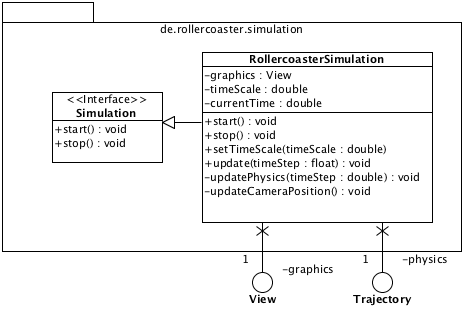
\includegraphics[width=\linewidth]{bilder/Simulation}
\caption{Simulation}
\end{figure}

\subsection{Erläuterung}

Obwohl die Simulator-Komponente den Kern der Anwendung darstellt, ist ihre Funktionalität
ziemlich einfach. Die Implementierung \emph{RollercoasterSimulation} lässt sich als
\emph{ViewObserver} über die Fortschritte bei der grafischen Darstellung informieren
und lässt in der Hilfsmethode \emph{updatePhysics} die Physik einen neuen Zustand 
der \emph{Trajectory} berechnen. Anschließend wird in der Hilfsmethode \emph{updateCamera}
die Grafik über die neue Kameraeinstellung informiert.

Der Simulator ermöglicht der Benutzeroberfläche den Zugriff auf die \textbf{Observer}-
Funktionalität der \emph{Trajectory}, in dem er die entsprechenen Methodenaufrufe durchreicht.
